\documentclass{article}
\usepackage{civ}

\title{CIV102: Quiz 1 \\ \textit{Note: Ignore all pencil markings on diagrams.}}
\author{}
\date{}
\usepackage{mathrsfs}
\usetikzlibrary{arrows}
\setlength{\parindent}{0cm}
\begin{document}

\maketitle
\section*{2007 Quiz}
\textbf{Question 1:} A nautical mile is the distance traveled in moving through one minute of latitude. A ship which is sailing at a speed of five knots travels five nautical miles in one hour. Two hundred years ago, the speed of a British naval vessel was determined by lowering a small sea anchor which was called a log, and then measuring the length of cable played out from the ship during a fixed period of time. The length of cable was measured in fathoms (one fathom equals six feet) and every eight fathoms a knot was placed in the cable. The speed might thus be recorded as ``three knots, two fathoms''. The measuring period was determined using a small sand-filled ``hour'' glass. What was the length of time used for the measurement? (1 foot = 305 mm)

\textbf{Question 2:} The Niagara River connects Lake Erie to Lake Ontario and drops a total vertical distance of $325$ feet. About half of this drop occurs as the water cascades over Niagara Falls. Approximately $60\%$ of the water flowing down the Niagara River is diverted around the falls and used to generate about $4.3$ million kilowatts of electricity. If one Joule is the energy created by a force of $1$ Newton moving through a distance of $1$ meter and one watt is the power generated by one Joule of energy in one second, then what is the approximate volume of the water flowing over Niagara Falls?

\newpage
\section*{2009 Quiz}
\subsection*{Version 1}
\textbf{Question 1:} On July 15th this year at 9:22pm a strong earthquake with magnitude of $7.8$ struck the South Island of New Zealand. The source of the earthquake (hypocenter) was located $12$ km under the sea bed at about 100 km south-west of Tuatapere (see the map). The ground shaking caused town clocks in Blenheim and Timaru to stop (see the photograph). According to a journalist reporting the earthquake, the two clocks shown below were out of sync because they stopped at times different from 9:22 pm. Answer the following questions:
\begin{enumerate}
    \item Is it possible that the journalist was wrong and why?
    \item What was the average velocity of propagation of the seismic waves from the source of the earthquake to the cities of Blenheim and Timaru?
    \item Were the two clocks really out of sync?
\end{enumerate}
\begin{center}
    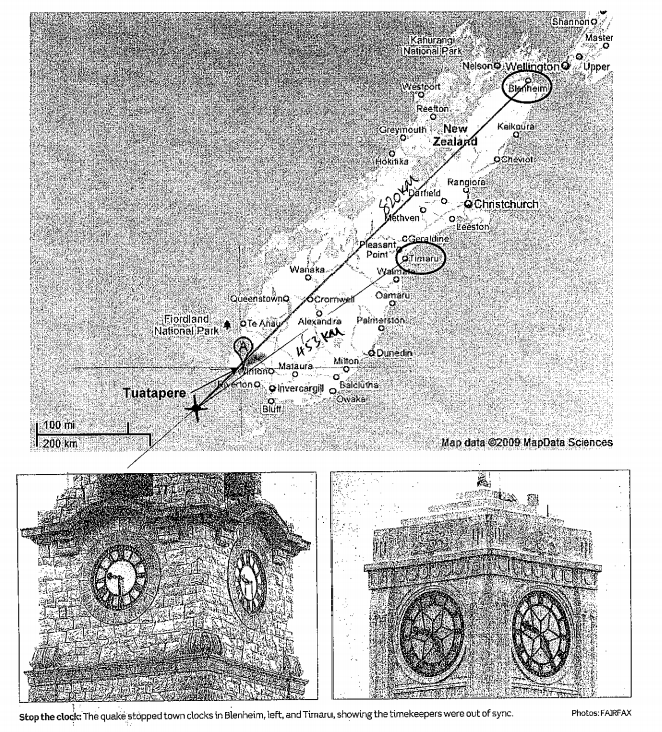
\includegraphics[width=0.8\linewidth]{2009-1-1.png}
\end{center}

\newpage
\textbf{Question 2:} In 1956, Frank Llyod Wright, then in his late 80s, presented his plans for the Illinois, a 528-story sky scraper that would have towered a full mile above Chicago. Shaped like a giant rapier, the steel and aluminum building would have provided office space for $100,000$ workers, parking for $15,000$ cars and landing decks for $150$ helicopters. Calculate how long it would take Chicago's rail system to deliver $100,000$ workers to the proposed skyscraper. Assume that a fully loaded eight-car train shown below arrived at the building every five minutes.
\begin{center}
    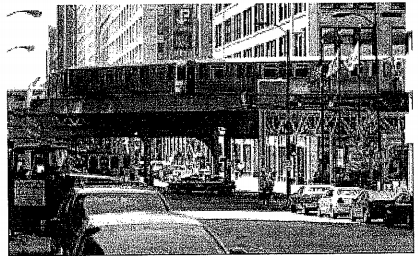
\includegraphics[width=0.8\linewidth]{2009-1-2.png}
\end{center}

\newpage
\subsection*{Version 2}
\textbf{Question 1:} The Great Laxey Wheel located in the Isle of Man in the Irish Sea is the largest surviving waterwheel in Europe. It was built in 1854 and it has been used to pump water out of a mine rich in lead and zinc. The wheel has a diameter of 22 meters and is powered by water gathered in a reservoir located 3 meters above the highest point of the wheel. The circular motion of the wheel is converted by a crank to horizontal motion of a system of horizontal rods. The horizontal motion of the rods, in turn, is converted by a ``T-rocker'' to vertical motion (up and down) of a vertical pump rod installed in one of the shafts of the mine. The water is pumped from the bottom of the shaft up 450 meters to a horizontal adit from where it is directed to the Laxey River. If you know that the pumps pump 1100 liters of water per minute, what is the water supply from the reservoir expressed in litres per minute? Assume that friction and other effects in the system result in $50\%$ of energy.
\begin{center}
    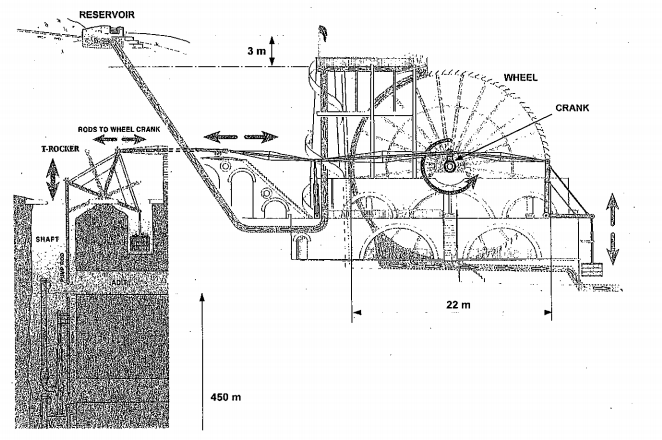
\includegraphics[width=0.8\linewidth]{2009-2-1.png}
\end{center}

\newpage
\textbf{Question 2:} Given below is the map of the island of Cyprus. Estimate the area of this island. State clearly any assumptions or approximations that you make.
\begin{center}
    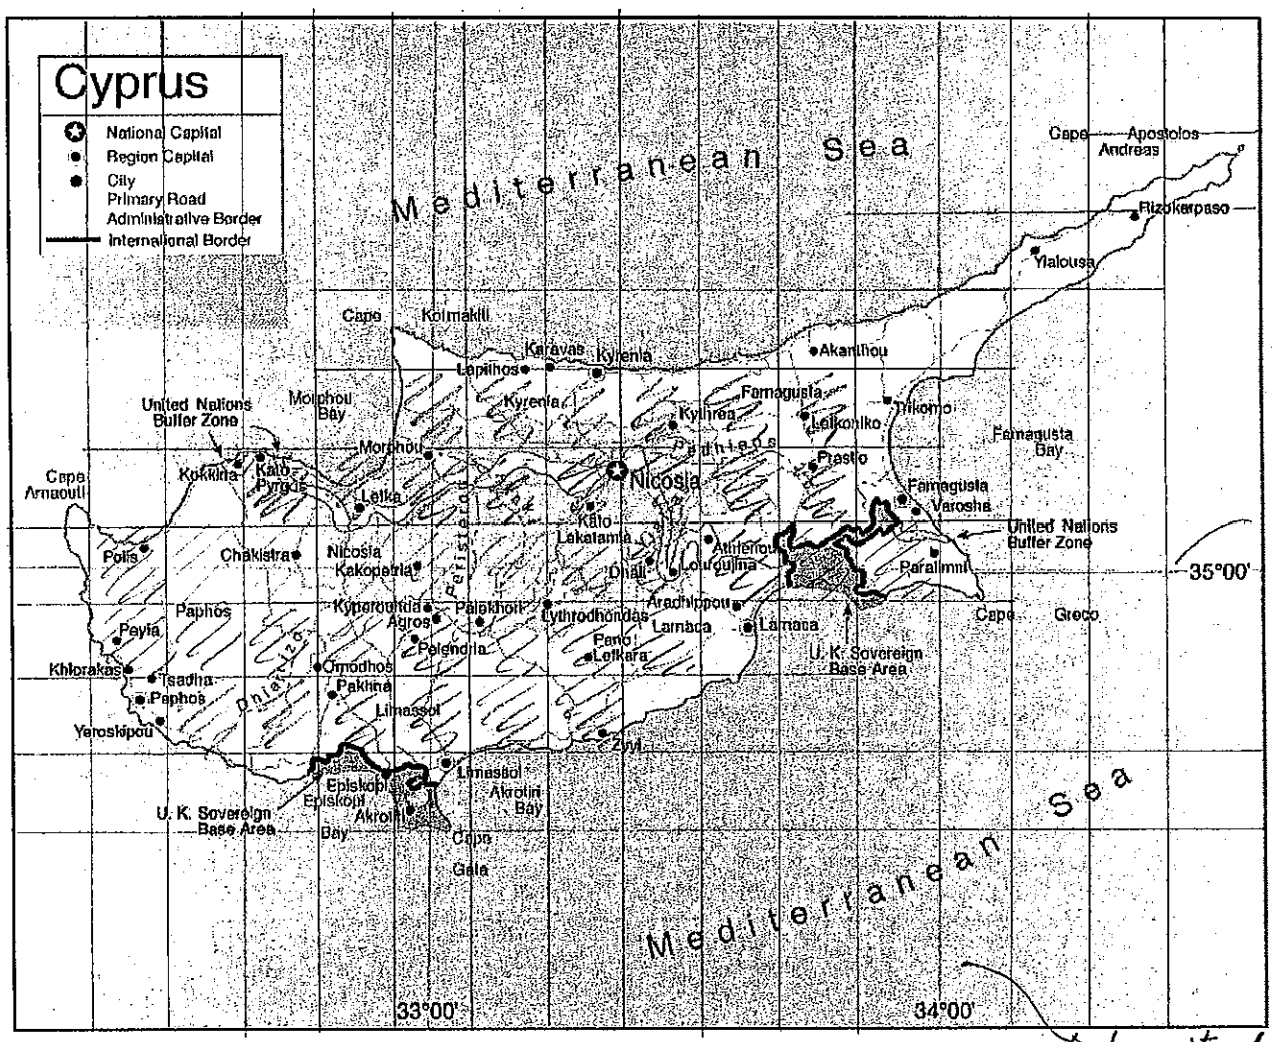
\includegraphics[width=0.8\linewidth]{2009-2-2.png}
\end{center}

\newpage
\subsection*{Version 3}
\textbf{Question 1:} In the initial surveys of Canada much of the land was divided into townships each 6 miles north-south on a side and 6 miles east-west. The townships were in turn subdivided into 36 ``sections'' each one mile by one mile. There was a road allowance one chain wide along each section line (80 chains = 1 mile). A typical farm was a quarter section that is 40 chains by 40 chains. Excluding the road allowances, how many acres did a farmer own who purchased a quarter section? One acre equals 10 square chains.
\begin{center}
    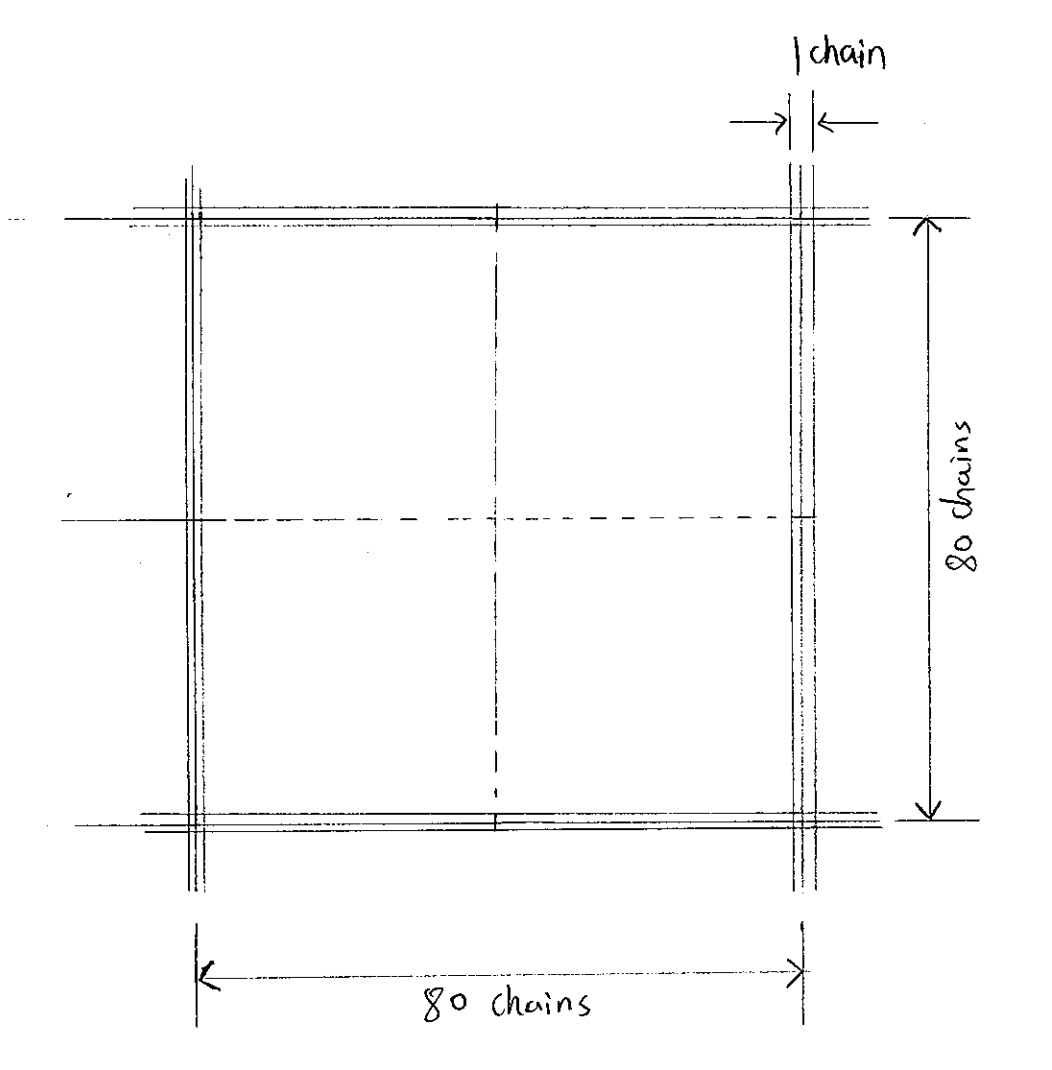
\includegraphics[width=0.8\linewidth]{2009-3-1.png}
\end{center}

\newpage
\textbf{Question 2:} You are evaluating the relative cost efficiency of fuel for proposed transportation options for a $110$ km route between Toronto and Waterloo: automobiles using gasoline, a natural gas powered bus, and a train using diesel fuel. Statistics about each vehicle are presented in the table below. The mass of each passenger can be taken as $90 \text{ kg}$. The number of daily travelers is 10,000. The service will operate Monday to Friday, including holidays. Determine the:
\begin{enumerate}
    \item cost of the best technology as a percentage of the worst cost.
    \item lowest annual operating cost of the technologies considered.
\end{enumerate}
\begin{center}
    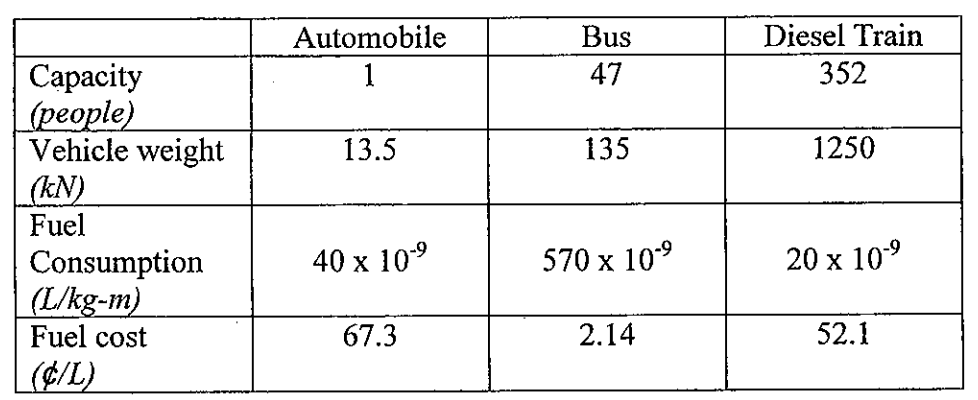
\includegraphics[width=0.8\linewidth]{2009-3-2.png}
\end{center}

\newpage
\section*{2011 Quiz}
\subsection*{Version 1}
\textbf{Question 1:} In the 1790's French engineers determined the distance from the North Pole to the Equator by measuring the distance of a North-South line from Dunkirk to Barcelona and by determining the latitudes of Dunkirk and Barcelona. Using the given map estimate the north-south distance from Dunkirk to Barcelona. If your distance was the value they also determined and if their measured latitude for Dunkirk was $51^\circ02'N$, what was their measured latitude for Barcelona? 
\begin{center}
    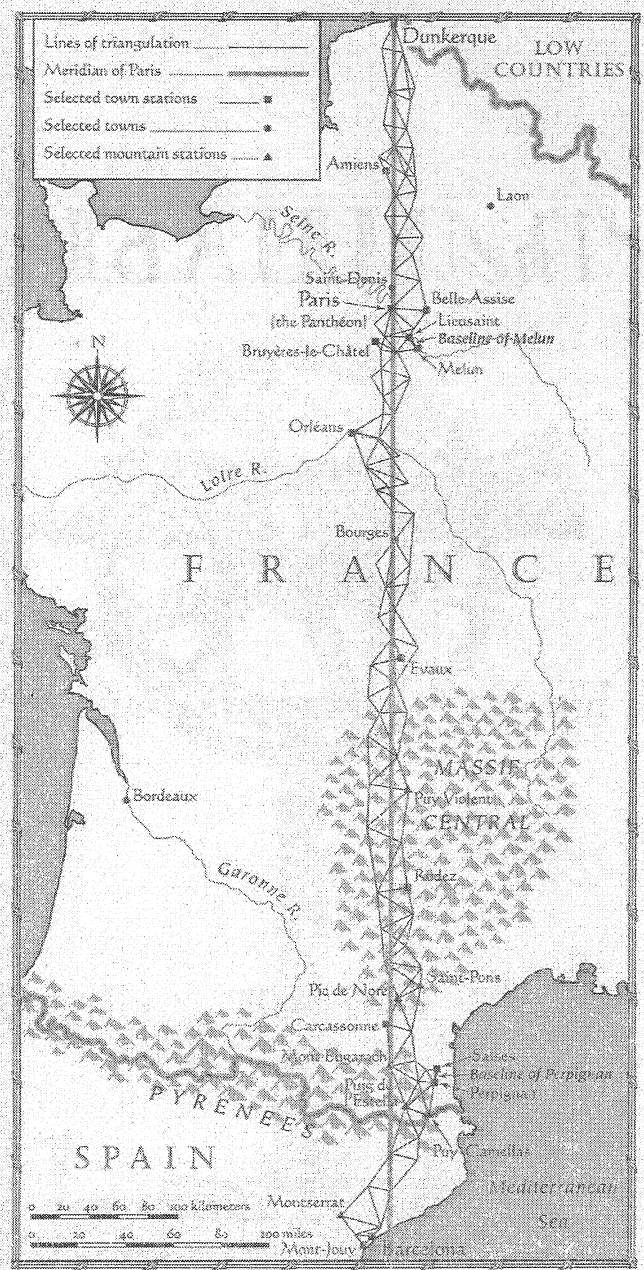
\includegraphics[width=0.5\linewidth]{2011-1-1.png}
\end{center}

\newpage
\textbf{Question 2:} Shown below is an elevation of the famous Pantheon in Rome built under Emperor Hadrian's direction in about $120$ AD.
\begin{enumerate}
    \item Estimate the total volume of air inside the Pantheon
    \item Estimate the energy required to raise the temperature of the air inside the Pantheon by $5^\circ \text{ C}$. The density of air is $1.2 \text{ kg/m}^3$ and 1000 Joules of energy will raise the temperature of $1$ kg of air by $1^\circ$C.
\end{enumerate}
\begin{center}
    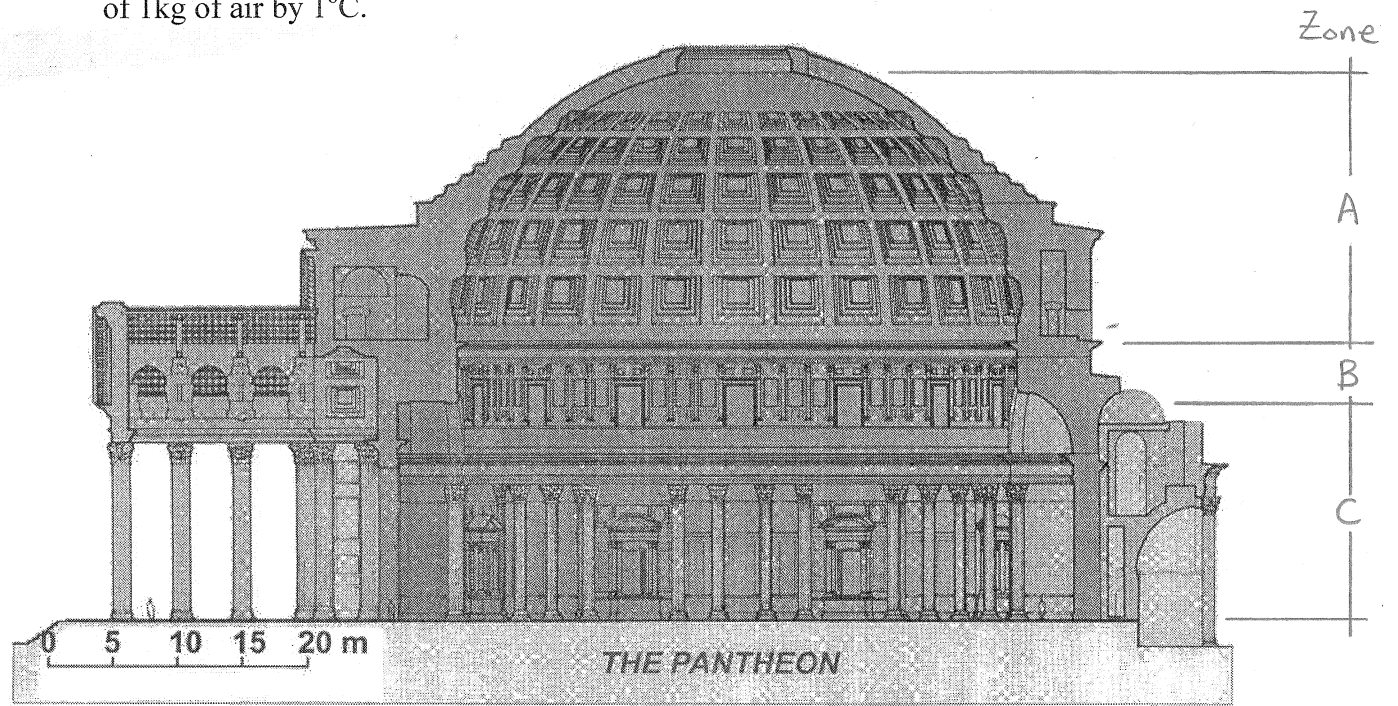
\includegraphics[width=0.5\linewidth]{2011-1-2.png}
\end{center}

\newpage
\subsection*{Version 2}
\textbf{Question 1:} The Tokyo Wan Aqua-Line (Trans-Tokya bay Highway) is a $15.1-$kilometer toll highway that runs across the central portion of Tokyo bay, connecting Kisarazu with Kawasaki by a $15-$minute drive. It consists of $4.4 \text{ km}$ of bridge starting from the Kisarazu side and roughly $9.5 \text{ km}$ of tunnel from the Kawasaki side. At the transition between the bridge and the tunnel portions lies Umi-hotaru (Kisarazu Man-made Island), and another man-made island named Kaze-no-to (Kawasaki Man-made Island) is located at the mid point of the tunnel. Kaze-no-to, a circular structure 195 m in diameter, consists of a diaphragm wall enclosed in steel jackets designed to absorb the shock of possible ship collisions.

The following equation represents the force that must be resisted by the artificial island as a ship collides into it.
$$F=5000(1-\cos(0.33D)) MN$$
But
$$F \le 7000 MN$$
where $F$ is the force exerted on the platform in MegaNewtons, $D$ is the distance the centre of gravity of the ship has moved in meters, and $0.33D$ has units of radians.
\begin{enumerate}
    \item Plot below the relationship between $F$ and $D$ for values of $D$ ranging from zero to $7$ meters.
    \item The kinetic energy (Joules) absorbed by the ship is the area under the curve. Calculate using the graph, the area under the curve between $D=0 \text{ m}$ and $D=7\text{ m}$.
    \item Using this energy and the equation that $\text{energy}=\frac{1}{2}mv^2$, calculate the initial speed a ship, that has a mass of 6 million tonnes, would have to have to push this far towards the island.
    \item Does this answer make sense?
\end{enumerate}
\begin{center}
    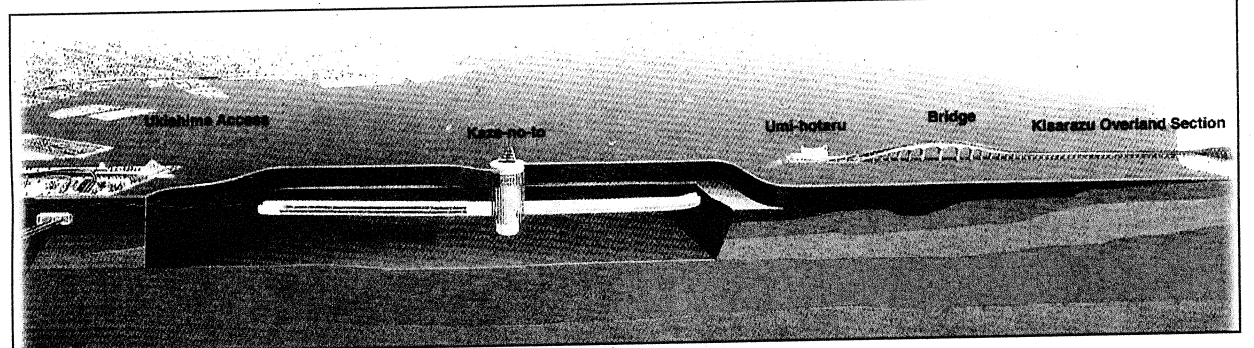
\includegraphics[width=0.8\linewidth]{2011-2-1.png}
\end{center}

\newpage
\textbf{Question 2:} About 500 years ago Leonardo da Vinci designed an extraordinary stone arch bridge with which he proposed to span the Golden Horn in Istanbul. The bridge was never built, but Da Vinci's vision was resurrected in 2011 when a smaller bridge based on his design was constructed in Norway. Shown in the picture below in the Norwegian Leonardo Bridge, which was opened to foot and bicycle traffic on October 31, 2001. Estimate the height of the bridge from the road. State clearly any assumptions or approximations that you make.
\begin{center}
    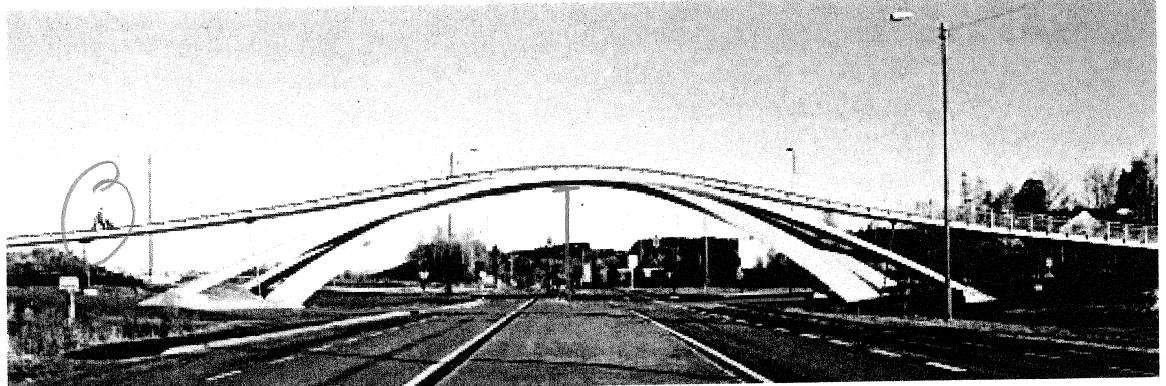
\includegraphics[width=0.8\linewidth]{2011-2-2.png}
\end{center}

\newpage
\subsection*{Version 3}
\textbf{Question 1:} In a thermometer, a material such as mercury is placed in a sphere with a small tube extending out. This sphere is used to measure small changes in volume accurately. As temperature rises, the mercury expands and rises higher in the tube. You have decided to build your own thermometer to check the weather and need to calibrate it. The bulb is $10 \text{ mm}$ in internal diameter and is shown below in a scale drawing. Calculate how much higher the mercury level will be after being placed in boiling water for a while. Comment on the design. The coefficient of thermal expansion of mercury is $180\times 10^{-6}$ mL expansion for mLof mercury per degree Celsius. You can assume the rate of expansion of the glass container is negligible in comparison to that of the mercury.
\begin{center}
    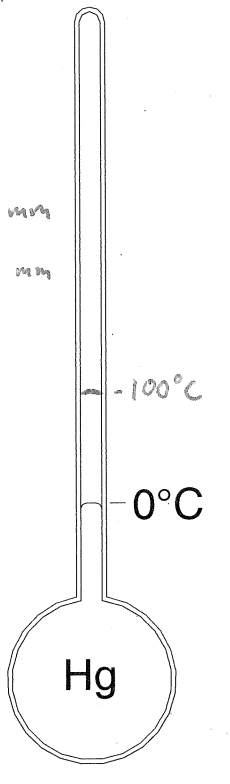
\includegraphics[width=0.3\linewidth]{2011-3-1.png}
\end{center}

\newpage
\textbf{Question 2:} Given below is the map of Tasmania. Estimate the area of the island.
\begin{center}
    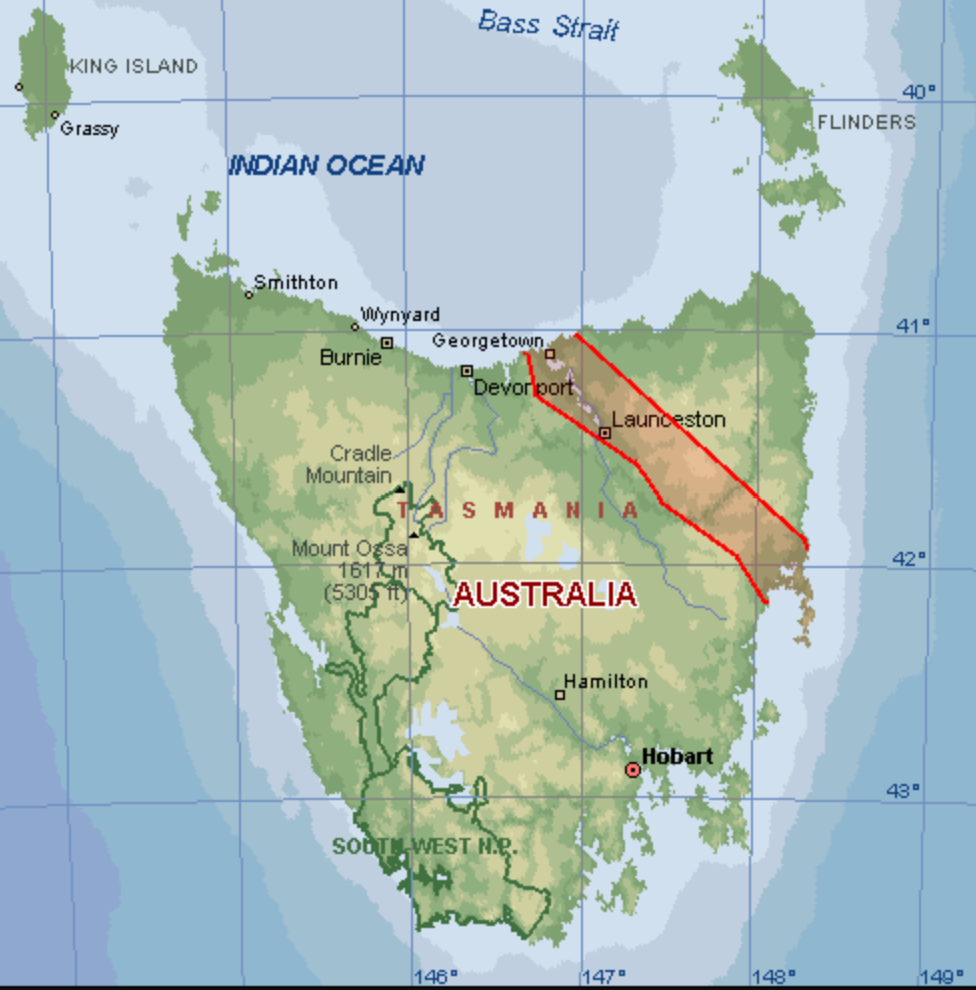
\includegraphics[width=0.8\linewidth]{2011-3-2.png}
\end{center}

\newpage
\section*{2019 Quiz}
\textbf{Question:} Shown on the opposite page is a schematic of the Golden Gate Bridge, located in San Francisco and built in 1937. Each of the two cables which support the deck consists of $27,572$ high strength steel wires wound together into a bundle. The diameter of the individual wires is $4.93 \text{ mm}$ and the unit weight of steel is $77 \text{ kN/m}^3$. Estimate the total weight of steel contained in the primary cables which hold up the bridge (i.e. ignore the vertical wires which connect the primary cables to the bridge deck). Report your answer in units of tonnes (1 tonne =1000 kg). See \href{https://www.goldengate.org/assets/1/6/ggb_plan_elevation_drawing.jpg}{diagram}.
\begin{center}
    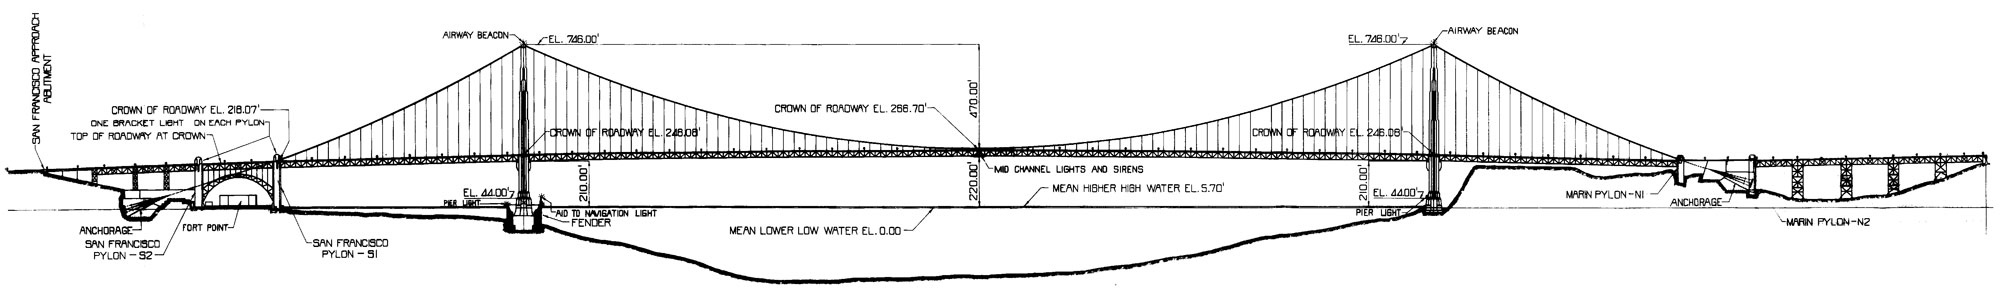
\includegraphics[width=\linewidth]{2018-1-1.jpg}
\end{center}
\end{document}
